%Micah Chambers

\documentclass{beamer}
\usepackage[orientation=landscape,size=custom,width=16,height=10,scale=0.5,debug]{beamerposter} 

\mode<presentation>
{
  \usetheme{VT}
  % or ...

  \setbeamercovered{transparent}
  % or whatever (possibly just delete it)
}

\usefonttheme[onlylarge]{structurebold}
\usecolortheme{crane}
\setbeamerfont*{frametitle}{size=\normalsize,series=\bfseries}
\setbeamertemplate{navigation symbols}{}
\setbeamercovered{transparent}


\usepackage[english]{babel}
% or whatever

\usepackage[latin1]{inputenc}
% or whatever

\usepackage{graphics}
\usepackage{times}
\usepackage[T1]{fontenc}
\usepackage[small]{caption}

\title{BOLD Parameter Estimation using Sequential Monte Carlo Methods}

%\subtitle{}

\author{Micah Chambers}

\institute {Virginia Tech Bioimaging Systems Lab}

\subject{Medical Imaging}

% If you have a file called "university-logo-filename.xxx", where xxx
% is a graphic format that can be processed by latex or pdflatex,
% resp., then you can add a logo as follows:

\pgfdeclareimage[width=1.5cm]{university-logo}{logo}
\logo{\pgfuseimage{university-logo}}


% If you wish to uncover everything in a step-wise fashion, uncomment
% the following command: 

%\beamerdefaultoverlayspecification{<+->}


\begin{document}
\begin{frame}
  \titlepage
\end{frame}

\begin{frame}{Outline}
  \tableofcontents
  % You might wish to add the option [pausesections]
\end{frame}

\section{FMRI Review}
\begin{frame}{The BOLD Response}
\begin{figure}
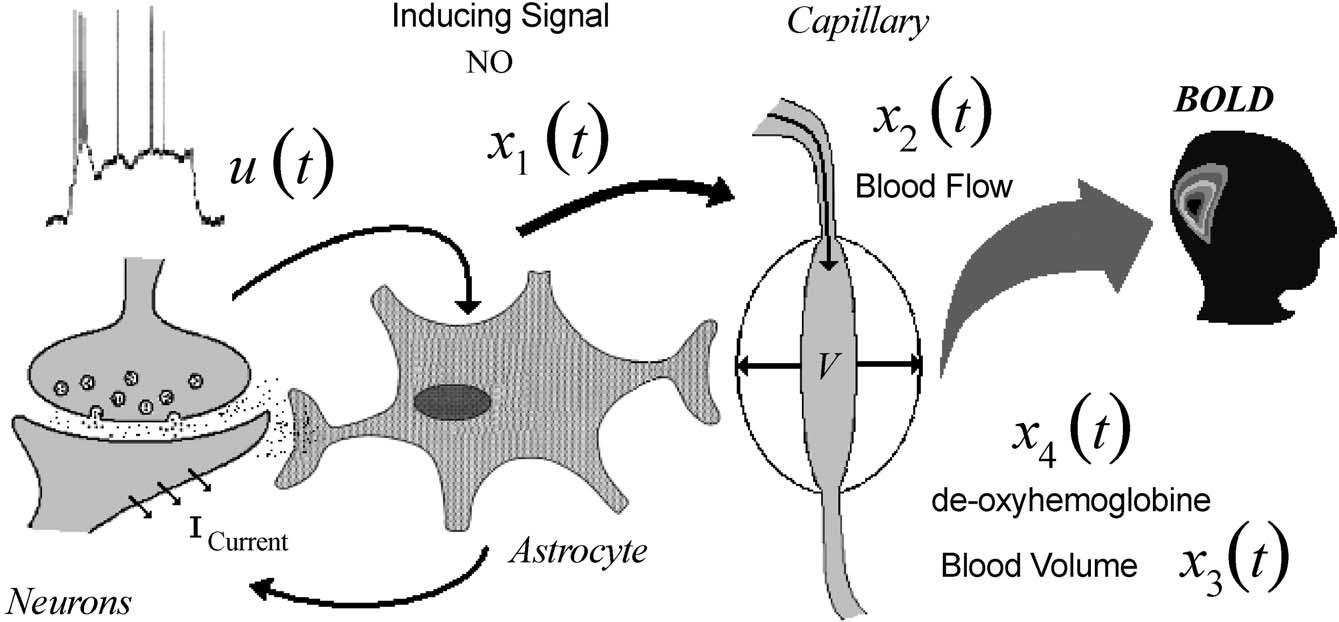
\includegraphics[scale=.23]{model}
\caption{
    \tiny
    \cite{ISI:000189252300007}
}
\end{figure}
\end{frame}

\begin{frame}{BOLD Signal Properties}
  \begin{itemize}
    \item Exact variables and parameters are unknown and are
        difficult to calculate.
    \item Significant Amount of Lag between activation
        and a measurable output - can be as much as 8 seconds.
    \item Slow Temporal Resolution
    \item Noise characterized by brownian motion
    \item fft of mri signal, with and without DC
  \end{itemize}
\end{frame}

\begin{frame}{Preprocessing}
  \begin{itemize}
    \item High Pass Filter and Low Pass Filter
    \item Wavelet Detrending
    \item ...
    \item Spline
  \end{itemize}
\end{frame}

\section{Statistical Parametric Mapping}
\begin{frame}{Method}
  \begin{itemize}
    \item
  \end{itemize}
\end{frame}

\begin{frame}{Results}
  \begin{itemize}
    \item ...
  \end{itemize}
\end{frame}

\begin{frame}{Limitations}
  \begin{itemize}
    \item ...
  \end{itemize}
\end{frame}

\section{Nonlinear Regression}
\begin{frame}{Equations}
  \begin{itemize}
    \item Normalized Cerebral Blood Flow:
    $$\ddot{f}(t) = \epsilon u(t) - \dot{f}(t)/\tau_s - (f(t)/\tau_f - 1)$$
    \item Normalized Cerebral Blood Volume:
    $$\dot{v}(t) = (1/\tau_0)( f(t) - v(t) ^ {1/\alpha}) $$
    \item Normalized Deoxyhaemoglobin Content:
    $$\dot{q}(t) = \frac{1}{\tau_0}\left(\frac{f(t)(1- (1-E_0)^{1/f(t)})}{E_0} - 
            \frac{q(t)}{v(t)^{1-1/\alpha}}\right)$$
    \item Hemodynamic Response - BOLD Signal
    $$y(t) = V_0(a_1( 1 - Q(t)) - a_2(1 - V(t)))$$
  \end{itemize}
\end{frame}

\begin{frame}{Alternative Equations}
\begin{itemize}
    \item The Balloon Model proposed by \cite{ISI:000073759600002} is the basic model.
    \item There are more complicated versions of the BOLD model:
    \begin{itemize}
        \item \cite{ISI:000240969200015} Reviews several existing models
        \item \cite{Buxton2004S220} Pioneered the Balloon model which was shown in the beginning.
        \item \cite{ISI:000234015300018} Adds interesting neural activation and a habituation model
        \item Some models loosen the link between CMRO2 (oxygen metabolism)
            and Cerebral Blood Flow - likely due to several papers that report
            such a decoupling.
    \end{itemize}
\end{itemize}
\end{frame}

\begin{frame}{Model Comparisons}
\begin{figure}
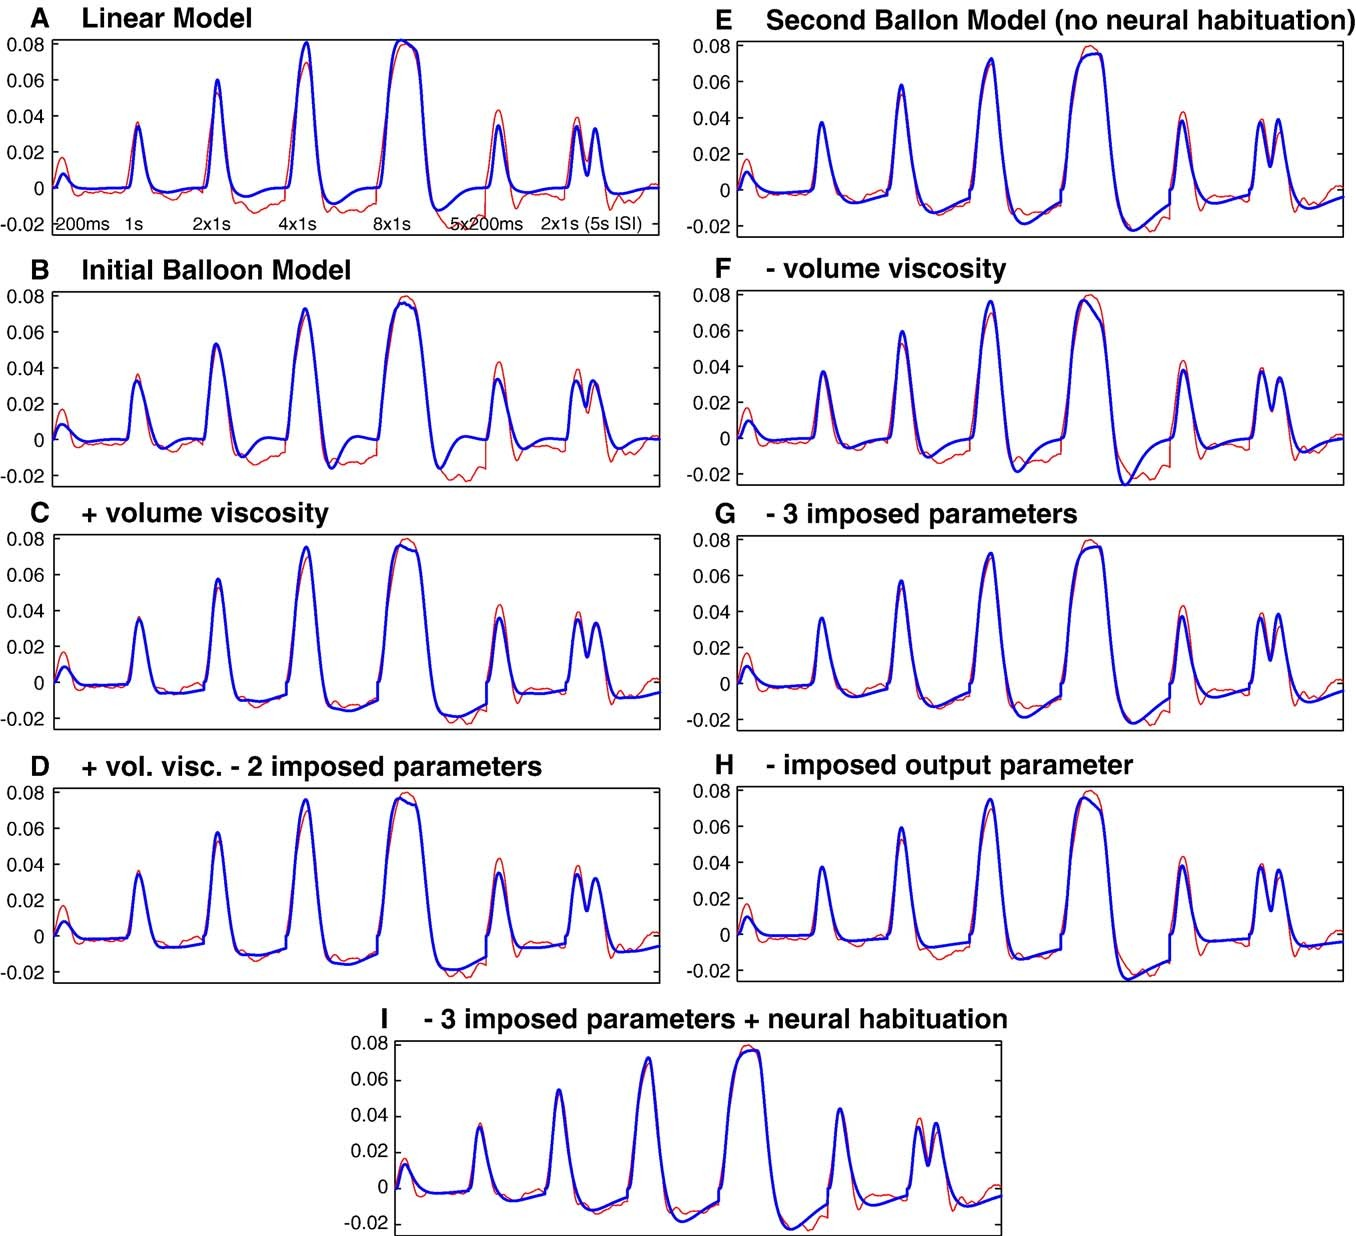
\includegraphics[scale=.165]{demeux}
\end{figure}
\end{frame}

\section{Parameter Identification}
\begin{frame}{Particle Filters}
\begin{itemize}
    \item Why Particle Filters
    \item Goal: $\epsilon$
    \item Entire brain
\end{itemize}
\end{frame}

\begin{frame}{Single Timeseries Results}
\end{frame}

\begin{frame}{Simulation}
\end{frame}

\begin{frame}{Simulation Results}
\end{frame}

\section{Conclusion}

% All of the following is optional and typically not needed. 
\appendix
\section<presentation>*{\appendixname}
\subsection<presentation>*{For Further Reading}

\begin{frame}[allowframebreaks]
  \bibliographystyle{abbrvnat}
  \bibliography{references}
\end{frame}

\end{document}



